
\documentclass[
   ngerman          % neue deutsche Rechtschreibung
  ,a4paper          % Papiergrösse
% ,twoside          % Zweiseitiger Druck (rechts/links)
% ,10pt             % Schriftgrösse
  ,11pt
% ,12pt
  ,pdftex
%  ,disable         % Todo-Markierungen auschalten
]{report}

% Bitte die Codierung Ihrer Dateien auswählen:
% \usepackage[latin1]{inputenc}    % Für UNIX mit ISO-LATIN-codierten Dateien
% \usepackage[applemac]{inputenc}  % Für Apple Mac
% \usepackage[ansinew]{inputenc}   % Für Microsoft Windows
\usepackage[utf8]{inputenc}        % UTF-8 codierte Dateien
                                   % Dieses Dokument ist unter Unix erstellt, daher
                                   % wird diese Input-Codierung benutzt.

\usepackage{bericht}
\usepackage[graphicx]{realboxes}

\usepackage{lscape}
\usepackage[inkscapelatex=false]{svg}

\csname endofdump\endcsname

%%%%%%%%%%%%%%%%%%%%%%%%%%%%%%%%%%%%%%%%%%%%%%%%%%%%%%%%%%%%%%%%%%%%%%%%%%%%%%%
%% Angaben zur Arbeit
%%%%%%%%%%%%%%%%%%%%%%%%%%%%%%%%%%%%%%%%%%%%%%%%%%%%%%%%%%%%%%%%%%%%%%%%%%%%%%%


\newcommand{\Autor}{Lorenz Scherrer}
\newcommand{\MatrikelNummer}{8809469}
\newcommand{\Kursbezeichnung}{tinf21b3}

\newcommand{\FirmenName}{SICK AG}
\newcommand{\FirmenStadt}{Waldkirch}
\newcommand{\FirmenLogoDeckblatt}{\fbox{
\includegraphics[width=3cm]{images/SICK_Logo_Claim}}}


\newcommand{\BetreuerFirma}{Manfred Haberer}
\newcommand{\BetreuerDHBW}{Prof. Dr. Jürgen Vollmer}

%%%%%%%%%%%%%%%%%%%%%%%%%%%%%%%%%%%%%%%%%%%%%%%%%%%%%%%%%%%%%%%%%%%%%%%%%%%%%%%%%%%%%

% Wird auf dem Deckblatt und in der Erklärung benutzt:
\newcommand{\Was}{Projektarbeit}


%%%%%%%%%%%%%%%%%%%%%%%%%%%%%%%%%%%%%%%%%%%%%%%%%%%%%%%%%%%%%%%%%%%%%%%%%%%%%%%%%%%%%

\newcommand{\Titel}{Aufbau eines virtuellen Umweltmodelles für die Entwicklungen von 
Algorithmen für die sichere Personenerkennung in Automated Guided Vehicle Appikatonen}
\newcommand{\AbgabeDatum}{24. September 2023}

\newcommand{\Dauer}{12 Wochen}

% \newcommand{\Abschluss}{Bachelor of Engineering}
\newcommand{\Abschluss}{Bachelor of Science}

\newcommand{\Studiengang}{Informationstechnik}
% \newcommand{\Studiengang}{Informatik / Angewandte Informatik}

\hypersetup{%%
  pdfauthor={\Autor},
  pdftitle={\Titel},
  pdfsubject={\Was}
}

%%%%%%%%%%%%%%%%%%%%%%%%%%%%%%%%%%%%%%%%%%%%%%%%%%%%%%%%%%%%%%%%%%%%%%%%%%%%%%%


% Benutzt man das "biblatex"-Paket, dann muß das hier stehen:
% siehe auch die mit BIBLATEX markierten Zeilen in bericht.sty
\bibliography{quellen}

%\setlength{\marginparwidth}{2cm}

\begin{document}

%%%%%%%%%%%%%%%%%%%%%%%%%%%%%%%%%%%%%%%%%%%%%%%%%%%%%%%%%%%%%%%%%%%%%%%%%%%%%%%

\begin{titlepage}
\begin{center}
\vspace*{-2cm}
\FirmenLogoDeckblatt\hfill
\includegraphics[width=4cm]{images/dhbw-logo}\\[2cm]
{\Huge \Titel}\\[1cm]
{\Huge\scshape \Was}\\[1cm]
{\large für die Prüfung zum}\\[0.5cm]
{\Large \Abschluss}\\[0.5cm]
{\large des Studienganges \Studiengang}\\[0.5cm]
{\large an der}\\[0.5cm]
{\large Dualen Hochschule Baden-Württemberg Karlsruhe}\\[0.5cm]
{\large von}\\[0.5cm]
{\large\bfseries \Autor}\\[1cm]
{\large Abgabedatum \AbgabeDatum}
\vfill
\end{center}
\begin{tabular}{l@{\hspace{2cm}}l}
Bearbeitungszeitraum	          & \Dauer 			        \\
Matrikelnummer	                & \MatrikelNummer		  \\
Kurs			                      & \Kursbezeichnung		\\
Ausbildungsfirma	              & \FirmenName			    \\
			                          & \FirmenStadt			  \\
Betreuer der Ausbildungsfirma	  & \BetreuerFirma		  \\
Gutachter der Studienakademie	  & \BetreuerDHBW		    \\
\end{tabular}
\end{titlepage}

%%%%%%%%%%%%%%%%%%%%%%%%%%%%%%%%%%%%%%%%%%%%%%%%%%%%%%%%%%%%%%%%%%%%%%%%%%%%%%%

%%%%%%%%%%%%%%%%%%%%%%%%%%%%%%%%%%%%%%%%%%%%%%%%%%%%%%%%%%%%%%%%%%%%%%%%%%%%%%%
%% Descr:       Vorlage für Berichte der DHBW-Karlsruhe, Erklärung
%% Author:      Prof. Dr. Jürgen Vollmer, vollmer@dhbw-karlsruhe.de
%% $Id: erklaerung.tex,v 1.11 2020/03/13 14:24:42 vollmer Exp $
%% -*- coding: utf-8 -*-
%%%%%%%%%%%%%%%%%%%%%%%%%%%%%%%%%%%%%%%%%%%%%%%%%%%%%%%%%%%%%%%%%%%%%%%%%%%%%%%

% In Bachelorarbeiten muss eine schriftliche Erklärung abgegeben werden.
% Hierin bestätigen die Studierenden, dass die Bachelorarbeit, etc.
% selbständig verfasst und sämtliche Quellen und Hilfsmittel angegeben sind. Diese Erklärung
% bildet das zweite Blatt der Arbeit. Der Text dieser Erklärung muss auf einer separaten Seite
% wie unten angegeben lauten.

\newpage
\thispagestyle{empty}
\begin{framed}
\begin{center}
\Large\bfseries Erklärung
\end{center}
\medskip
\noindent
% siehe §5(3) der \enquote{Studien- und Prüfungsordnung DHBW Technik} vom 29.\,9.\,2017 und Anhang 1.1.13
Ich versichere hiermit, dass ich meine \Was mit dem Thema:
\enquote{\Titel}
selbstständig verfasst und keine anderen als die angegebenen Quellen und Hilfsmittel benutzt habe. Ich versichere zudem, dass die eingereichte elektronische Fassung mit der gedruckten Fassung übereinstimmt.
\vspace{3cm}
\noindent
\underline{\hspace{4cm}}\hfill\underline{\hspace{6cm}}\\
Ort~~~~~Datum\hfill Unterschrift\hspace{4cm}
\end{framed}

\vfill
\emph{Sofern  vom Dualen Partner ein Sperrvermerk gewünscht wird, ist folgende Formulierung
zu verwenden:}
\begin{framed}
\begin{center}
\Large\bfseries Sperrvermerk
\end{center}
\medskip
\noindent
Der Inhalt dieser Arbeit darf weder als Ganzes noch in Auszügen Personen
außerhalb des Prüfungsprozesses und des Evaluationsverfahrens zugänglich gemacht
werden, sofern keine anderslautende Genehmigung vom Dualen Partner vorliegt.
\end{framed}

%%%%%%%%%%%%%%%%%%%%%%%%%%%%%%%%%%%%%%%%%%%%%%%%%%%%%%%%%%%%%%%%%%%%%%%%%%%%%%%
\endinput
%%%%%%%%%%%%%%%%%%%%%%%%%%%%%%%%%%%%%%%%%%%%%%%%%%%%%%%%%%%%%%%%%%%%%%%%%%%%%%%


%%%%%%%%%%%%%%%%%%%%%%%%%%%%%%%%%%%%%%%%%%%%%%%%%%%%%%%%%%%%%%%%%%%%%%%%%%%%%%%

\newpage
\pagenumbering{Roman}
\tableofcontents           % Inhaltsverzeichnis hier ausgeben
\listoffigures             % Liste der Abbildungen
\listoftables              % Liste der Tabellen
\lstlistoflistings         % Liste der Listings
\listofequations           % Liste der Formeln

% Jetzt kommt der "eigentliche" Text
%%%%%%%%%%%%%%%%%%%%%%%%%%%%%%%%%%%%%%%%%%%%%%%%%%%%%%%%%%%%%%%%%%%%%%%%%%%%%%
%% Descr:       Vorlage für Berichte der DHBW-Karlsruhe, Datei mit Abkürzungen
%% Author:      Prof. Dr. Jürgen Vollmer, vollmer@dhbw-karlsruhe.de
%% $Id: abk.tex,v 1.4 2017/10/06 14:02:03 vollmer Exp $
%% -*- coding: utf-8 -*-
%%%%%%%%%%%%%%%%%%%%%%%%%%%%%%%%%%%%%%%%%%%%%%%%%%%%%%%%%%%%%%%%%%%%%%%%%%%%%%%

\chapter*{Abkürzungsverzeichnis}                   % chapter*{..} -->   keine Nummer, kein "Kapitel"
						         % Nicht ins Inhaltsverzeichnis
% \addcontentsline{toc}{chapter}{Akürzungsverzeichnis}   % Damit das doch ins Inhaltsverzeichnis kommt

% Hier werden die Abkürzungen definiert
\begin{acronym}[DHBW]
  % \acro{Name}{Darstellung der Abkürzung}{Langform der Abkürzung}
 \acro{Abk}[Abk.]{Abkürzung}

 % Folgendes benutzen, wenn der Plural einer Abk. benöigt wird
 % \newacroplural{Name}{Darstellung der Abkürzung}{Langform der Abkürzung}
 \newacroplural{Abk}[Abk-en]{Abkürzungen}

 \acro{H2O}[\ensuremath{H_2O}]{Di-Hydrogen-Monoxid}

 % Wenn neicht benutzt, erscheint diese Abk. nicht in der Liste
 \acro{NUA}{Not Used Acronym}
\end{acronym}
              % Abkürzungsverzeichnis
\newpage

\newcounter{savepage}
\setcounter{savepage}{\value{page}}
\pagenumbering{arabic}

\chapter{Einleitung}
%Beschreibe den Hintergrund und die Motivation deiner Arbeit. Erkläre, warum dieses Thema wichtig ist und welche Forschungsfragen du untersuchst.
Das Ziel dieser Abreit ist es ein virtuelle Umgebung zu erstellen um für die Entwicklung von Algorithmen für die sichere Personenerkennung in Automated Guided Vehicle. 
%Verstehe das Problem
Es sollen Umweltdaten von Automated Guided Vehicle Applikationen zur Entwicklung generiert werden. Die Umweltdaten sollen zum testen und Validieren von Sicherheitskonzepten. So sollen Worst-Case-Szenarien definiert werden und die Robustheit der Softwarealgorithemen geprüft werden.\\

Der Vorteil ist es das so viele mehr testdaten generiert werden könne ohne aufwendige Test Scenerien in einer realen Werkshalle aufzubauen.\\
%Identifiziere das Problem
%Hintergrundinformationen
%Relavanz betonen
%Ziele und Hypothesen
%Betonung des Neuigkeitswertes
%Zusammenfassung
%Zusätliche Quellen

%\section{Projektumfeld und Kontext}% kann auch weg gelassen werden
%GICTICIISM
%Global Industry Centers Technical Industry Competence \& Innovation

\section{Problemstellung}
%Verständnis des Themas: Stelle sicher, dass du ein klares Verständnis für das Thema deiner Arbeit hast, bevor du die Problemstellung formulierst.
%Identifikation des Problems: Überlege, welche spezifische Frage oder Herausforderung du in deiner Arbeit angehen möchtest. Welche Lücke in der bestehenden Forschung möchtest du schließen oder welches Problem möchtest du lösen?
%DSM Project was ist dieses Projekt?
Die Problemstellung bindet sich im DSM ein. Es sollen die Sceneie aufgebaut werden und die Sensordaten dem gRPC Server bereitgestellten werden.
\begin{figure}[htp]
    \centering
    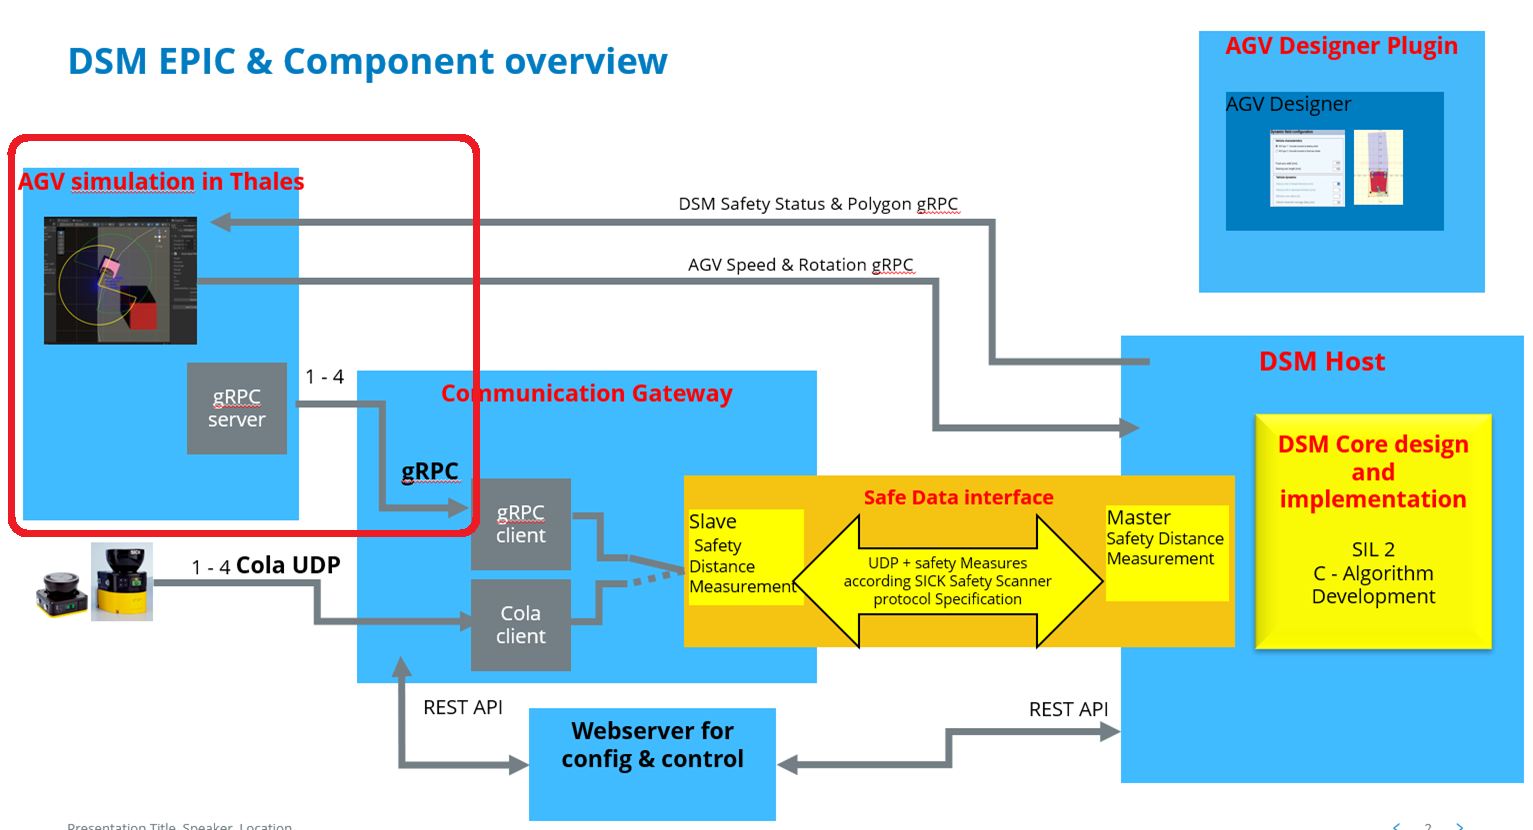
\includegraphics[width=(\textwidth)]{images/AGV_Overview.png}
    \caption{DSM EPIC \& Component overview}
    \label{fig:DSMoverview}
\end{figure}
%Wo finde ich informationen zum DSM Projekt? Boris morgen fragen
%Was trage ich zu deisem Projekt bei?

%Identifiziere die Lücke im Wissen:
Es gib keine Simulation in der man Gefahrensitzuationen testen kann. Ohne Sie in echten Hallen zu testen.
%Spezifische Fragestellung: Formuliere deine Problemstellung als eine klare Frage. Diese Frage sollte präzise, klar und relevant sein. Vermeide vage oder mehrdeutige Formulierungen.


%Bedeutung und Relevanz Betone die Bedeutung deiner Problemstellung. Warum ist es wichtig, diese Frage zu beantworten oder dieses Problem zu lösen? Welche Auswirkungen könnte die Antwort haben?
Im weiteren verlauf kann der Algorithmus der die Sicherheitsfelder der AGVs berechnet an ein Instutut geschickt werden der diesen Valiediert. Oder ein in der Simulation getesten Algorithmus in echten Szenarien getestet werden.
Hier können die Sicherheitsalghrutmen erstmals getestet werden.

%Abgrenzung und Kontext: Kläre den Rahmen deiner Problemstellung. Welche Aspekte deines Themas wirst du behandeln und welche wirst du bewusst außer Acht lassen? Definiere den Kontext, in dem deine Fragestellung relevant ist.


\section{Zielsetzung}
%Die Zielsetzung beschreibt das übergeordnete Ziel deiner Arbeit. Sie verdeutlicht, was du mit deiner Forschung erreichen möchtest.
%Konkretheit: Formuliere deine Zielsetzung so konkret wie möglich. Vermeide allgemeine Formulierungen, die mehrdeutig sind.
%Messbarkeit: Stelle sicher, dass dein Ziel messbar ist. Das bedeutet, dass du später überprüfen können solltest, ob du es erreicht hast.
%Realistisch: Deine Zielsetzung sollte realistisch sein und in einem angemessenen Rahmen erreichbar sein.
%Relevanz: Betone, warum dein Ziel wichtig ist und welche Bedeutung es für die Forschung oder die Praxis hat.
Daten übermittel und ein AGv in Unity erstellen.

\section{Fragestellung}
%Die Forschungsfrage konkretisiert deine Zielsetzung und gibt die Richtung für deine Untersuchung vor. Sie sollte präzise, klar und offen genug sein, um die Möglichkeit zur Forschung zu bieten.
%Klarheit: Formuliere die Forschungsfrage klar und verständlich. Vermeide komplexe Satzstrukturen.
%Ein Frageaspekt: Fokussiere auf einen bestimmten Aspekt des Themas. Eine zu breite Fragestellung kann zu unübersichtlichen Ergebnissen führen.
%Beantwortbarkeit: Stelle sicher, dass deine Forschungsfrage durch deine Forschungsmethoden und Daten beantwortbar ist.

Wie kann ein AGV in Unity in erstellt werden und dessen Meschanische Daten über gRPC mit der Ausenwelt geteilt werden und auch Daten erhalten? 
\chapter{Planung und Kontrolle}


\section{Zeitmanagament}
%Einführung zur Zeitplanung
%1.1 Bedeutung einer strukturierten Zeitplanung
%1.2 Zielsetzung des Kapitels

\subsection{Meilensteinen und Etappen}
%2.1 Klare Definition von Forschungszielen und Teilzielen
%Erste Meilenstein Prio 1
%Der erste Meilenstein ist es die Schnittstelle über den gRPC Server und Client soll in beide richtungen Daten übertragen.
%Die Thales Sensordaten von 4 Sensoren müssen über den gRPC Server vom Client abgefragt werden können. Zur Aufnahme Zeit aber mindestens alle 40ms. 
Innerhalb ersten Meilensteins liegt der Fokus auf der Umsetzung einer funktionsfähigen Schnittstelle zwischen dem gRPC Server und Client, um Daten in beiden Richtungen zu übertragen. \\
Ein zentrales Ziel ist es, Thales Sensordaten von insgesamt 4 Sensoren über den gRPC Server vom Client abrufen zu können. Die Datenabfrage sollte in der Lage sein, mit einer Aufnahmefrequenz von mindestens alle 40 Millisekunden durchgeführt zu werden.\\
%Über den gRPC Server sollen auch andere Parameter übertragen werden wie Lenkwinkel oder Geschwindigkeit einer im späteren verlauf erstellten AGVs.
Zusätzlich zu den Sensordaten sollen auch andere Parameter über den gRPC Server übertragen werden, wie beispielsweise der Lenkwinkel oder die Geschwindigkeit eines zukünftig erstellten AGVs. Dieser Meilenstein bildet einen wesentlichen Schritt, um die grundlegende Funktionalität des Projektes zu etablieren und legt den Grundstein für die weitere Entwicklung im Projektverlauf.\\
%Zweiter Meilenstein Prio 2
%Der zweite Meilenstein soll die Umsetzung der AGVs enthalten. Dazu muss die Fahrphysik erstellt werden. Es sollten mehrer Arten von Agvs entwickelt werden aber mindestens eins. Zunächsten sollen ein AGVs nach einem normalen Auto erstellt werden dann ein Gabelstapler also ein dreiRad und dannach eine Panzerrolle in dieser Reinfolge.
Der Meilenstein umfasst die Erstellung der Fahrphysik für die AGVs. Dies beinhaltet die Realisierung von realistischen Bewegungsabläufen und Steuerungsmechanismen, die den Charakter der jeweiligen AGV-Typen authentisch wiedergeben.\\
Innerhalb dieses Meilensteins ist die Entwicklung mehrerer Arten von AGVs geplant, wobei mindestens eine Variante umgesetzt wird. In der Anfangsphase werden verschiedene AGVs entworfen, darunter ein AGV, das auf einem herkömmlichen Auto basiert, gefolgt von einem dreirädrigen Gabelstapler und schließlich einer Panzerrolle.\\
%Die Steuerung oder Fahranweisung soll über ein Script in Unity laufen welches sagt geschwindigkeit/Beschleunigung gibt und Lenkeinschlag der steuerachse
Die Steuerung und Fahranweisung der AGVs wird über ein Script in der Unity-Umgebung gesteuert. Dieses Script gibt die Geschwindigkeit, Beschleunigung und den Lenkeinschlag der Steuerachse vor.\\

Die erfolgreiche Umsetzung dieses Meilensteins wird die Basis für die funktionale und realistische Integration der AGVs in das Forschungsprojekt legen. Durch die Entwicklungsarbeit im zweiten Meilenstein wird die Grundlage für weiterführende Tests und Analysen der AGVs geschaffen, die zur Erreichung der gesamten Projekts beitragen.\\

%Dritter Meilenstein Prio 3 Dritter Meilenstein: Erfassung des AGV-Bremswegs als Polygonzug
%Im Dritten Meilenstein solle ein Polygonzug erhalten werden der den Bremsweg des AGVs wiederspielt. Er kann dierkt an erhalten werden jedoch muss noch überprüft werden ob es möglich ist ihn zu übertragen oder ob einfach die die länge des bremsschlauchs und darus mit dem lenkeinschlag der Bremsweg darstellt wird.
Innerhalb dieses Meilensteins ist das Hauptziel die Erstellung eines Polygonzugs, der den Bremsweg des AGVs abbildet. Dieser Polygonzug soll den Verlauf des Bremsvorgangs in einer geometrischen Darstellung wiedergeben.\newline
Nach der Erstellung des Polygonzugs muss überprüft 
werden, ob dieser direkt auf das AGV-Modell übertragen werden kann. Es ist von Bedeutung zu ermitteln, ob die Daten des Polygonzugs in das Simulationssystem eingeführt werden können, um eine korrekte Darstellung des Bremsverhaltens zu ermöglichen.\newline
Falls eine direkte Übertragung des Polygonzugs nicht möglich ist, wird eine alternative Methode in Betracht gezogen. Hierbei wird die Länge des Bremsschlauchs in Verbindung mit dem Lenkeinschlag genutzt, um den Bremsweg auf eine plausible Weise darzustellen.\newline
Die erfolgreiche Erfassung des AGV-Bremswegs als Polygonzug oder über alternative Darstellungsformen wird eine wichtige Grundlage für die Simulation des Bremsverhaltens in späteren Forschungsphasen bilden. Dieser Meilenstein trägt dazu bei, das Verhalten des AGVs unter verschiedenen Bedingungen besser zu verstehen und die Gesamtfunktionalität des Modells zu verbessern.\\

%Der vierte Meilenstein soll dafür sorgen das das Agv durch ein Siganl vom gRPC Client abbremst
Im Rahmen dieses Meilensteins wird das Hauptziel verfolgt, die Signalübertragung vom gRPC-Client zum AGV zu implementieren. Das Signal soll die Abbremsung des AGVs auslösen, wenn es empfangen wird.\\
Es ist von entscheidender Bedeutung, die Steuerungsfunktion im AGV zu konfigurieren, damit sie auf das empfangene Signal reagiert und die notwendigen Maßnahmen zur Abbremsung einleitet.\\
Die erfolgreiche Umsetzung dieses Meilensteins wird die Fähigkeit des AGVs zur externen Steuerung und zur Initiierung einer Abbremsung über das gRPC-Client-Signal demonstrieren. Diese Funktionalität kann im weiteren Verlauf der Forschungsarbeit dazu verwendet werden, verschiedene Szenarien und Anwendungen zu testen, bei denen eine externe Steuerung des AGVs erforderlich ist.\\
%2.2 Identifikation von wichtigen Meilensteinen im Forschungsprozess

%2.3 Unterteilung des Projekts in überschaubare Etappen
\subsection{Zeitplan}
%Erstellung eines Zeitplans
%3.1 Festlegung von Start- und Enddatum des Projekts
Das Projekt startet am 3. Juli und die Abgabe der schriftlichen Projektarbeit ist am 21. September. Nach der Berücksichtungen der Abwesenheiten umfasst das Projekt 35 Arbeitstage.

%3.2 Strukturierung des Zeitplans nach Etappen und Meilensteinen
In den ersten fünf Tagen des Projekts steht die Vorbereitung und Planung im Vordergrund. Hierbei werden die genauen Anforderungen und Ziele des Projekts geklärt. Es erfolgt eine detaillierte Aufschlüsselung der Arbeitsschritte sowie die Definition der benötigten Ressourcen.\\
Vom sechsten bis zum fünfzehnten Tag wird der erste Meilenstein erreicht - die Implementierung der gRPC-Server-Client-Schnittstelle. Ziel ist es, die bidirektionale Datenübertragung zwischen dem Server und Client zu ermöglichen.\\
Vom sechzehnten bis zum einundzwantigsten Tag liegt der Fokus auf dem zweiten Meilenstein, der die Umsetzung der AGVs beinhaltet. Es wird die Fahrphysik für verschiedene AGV-Typen erstellt, beginnend mit einem AGV, das sich wie ein herkömmliches Auto verhält. Die Bewegungsabläufe und Steuerung werden getestet und optimiert.\\
Vom zweiundzwanzigsten bis zum sechsundzwanzigsten Tag wird die Umsetzung der AGVs fortgesetzt. Ein Gabelstapler-AGV wird entwickelt, um dreirädrige Bewegungen zu simulieren. Parallel dazu wird die Vorbereitung für die Umsetzung des dritten AGV-Typs, einer Panzerrolle, getroffen.\\
Vom siebenundzwanzigsten bis zum neunundzwanzigsten Tag wird der dritte Meilenstein erreicht. Ein Polygonzug wird erstellt, um den Bremsweg des AGVs darzustellen. Die Übertragbarkeit dieser Daten auf das Modell wird geprüft, alternativ wird die Berechnung des Bremswegs anhand des Bremsschlauchs in Betracht gezogen.\\
Die letzten beiden Tage, der dreißigste und der zweidreißigste Tag, widmen sich dem vierten Meilenstein. Hierbei steht die Implementierung der externen Abbremsung des AGVs durch ein Signal vom gRPC-Client im Fokus. Die Steuerungsfunktion im AGV wird entsprechend konfiguriert und getestet, um sicherzustellen, dass das AGV zuverlässig auf das Signal reagiert.\\
%3.3 Berücksichtigung von Pufferzeiten für unvorhergesehene Verzögerungen

%Gantt-Diagramme und Visualisierung
%4.1 Verwendung von Gantt-Diagrammen zur grafischen Darstellung des Zeitplans
%4.2 Einfache Veranschaulichung von Aufgaben, Dauer und zeitlichen Abhängigkeiten

%Abhängigkeiten und Priorisierung
%6.1 Erkennen von Aufgabenabhängigkeiten und Verknüpfungen
%6.2 Priorisierung von Aufgaben basierend auf ihrer Relevanz und Abhängigkeit

%Überwachung und Anpassung des Zeitplans
%7.1 Regelmäßige Überprüfung des Fortschritts im Vergleich zum Zeitplan
%7.2 Identifizierung von Abweichungen und Verzögerungen
%7.3 Anpassung des Zeitplans bei Bedarf unter Berücksichtigung der Gesamtziele


\section{Risikoanalyse}


%Identifikation von Risiken
%2.1 Systematische Erfassung möglicher Risiken im Forschungsprozess
%2.2 Kategorisierung der Risiken (technische, organisatorische, finanzielle etc.)
%2.3 Einbeziehung von Stakeholdern zur Identifizierung potenzieller Risiken

%Bewertung von Risiken
%3.1 Einschätzung der Eintrittswahrscheinlichkeit für jeden identifizierten Risikofaktor
%3.2 Bewertung der Auswirkungen eines Risikos auf das Forschungsprojekt
%3.3 Kombination von Eintrittswahrscheinlichkeit und Auswirkungen zur Risikobewertung

%Priorisierung von Risiken
%4.1 Klassifizierung der Risiken nach ihrer Bedeutung (hoch, mittel, niedrig)
%4.2 Identifikation von kritischen Risiken, die besonders aufmerksam behandelt werden müssen

%Risikobewältigung und -managementstrategien
%5.1 Vorbeugende Maßnahmen zur Reduzierung der Eintrittswahrscheinlichkeit
%5.2 Minderungsstrategien zur Verringerung der Auswirkungen von Risiken
%5.3 Erstellung eines Aktionsplans zur Bewältigung prioritärer Risiken

%Kontinuierliches Monitoring und Anpassung
%6.1 Regelmäßige Überwachung der identifizierten Risiken
%6.2 Anpassung der Managementstrategien basierend auf neuen Erkenntnissen
%6.3 Berücksichtigung von Veränderungen im Forschungsprozess und der Umgebung


\chapter{Grundlagen}
\section{gRPC in Unity}
%Was ist das RPC Protokoll?
RPC steht für "Remote Procedure Call" (zu Deutsch: "Fernprozeduraufruf"). Es handelt sich um ein Protokoll und ein Konzept in der Informatik, das es ermöglicht, Funktionen oder Methoden auf entfernten Computern oder Prozessen aufzurufen, als ob sie auf dem lokalen Computer ausgeführt würden. RPC ermöglicht die Kommunikation zwischen verteilten Systemen und wird häufig in Client-Server-Anwendungen, Netzwerkdiensten und verteilten Systemen eingesetzt.\cite{Bengel.2004}\\

\begin{wrapfigure}{r}{0.25\textwidth} %this figure will be at the right
    \centering
    
\includegraphics[width=0.25\textwidth]{images/grpc-icon-color.png}
\end{wrapfigure}
Die Grundidee hinter RPC ist, dass ein Client-Programm eine Funktion oder Methode auf einem entfernten Server aufruft, als ob sie lokal vorhanden wäre. Der RPC-Mechanismus kümmert sich um die Details der Kommunikation, der Datenübertragung und der Rückgabewerte. Der Aufruf einer entfernten Funktion ähnelt daher stark einem normalen Funktionsaufruf in der Programmierung.\cite{Bengel.2004}\\

RPC erleichtert die Entwicklung von verteilten Anwendungen, da Entwickler sich nicht um die Details der Netzwerkkommunikation kümmern müssen. Es gibt verschiedene RPC-Implementierungen und Protokolle, darunter gRPC, XML-RPC, JSON-RPC und andere, die in verschiedenen Umgebungen und Anwendungsfällen eingesetzt werden können.\cite{Bengel.2004}\\

%Was ist gRPC?

gRPC ist ein leistungsstarkes Remote Procedure Call (RPC)-Framework, das von Google entwickelt wurde. Es wird häufig in verteilten Systemen und Microservices-Architekturen verwendet, um die Kommunikation zwischen verschiedenen Diensten zu erleichtern.\\

Eine der herausragenden Eigenschaften von gRPC ist die Verwendung des HTTP/2-Protokolls als Transportmechanismus. HTTP/2 bietet signifikante Verbesserungen gegenüber HTTP/1.x, darunter die Möglichkeit, mehrere Anfragen und Antworten über eine einzige TCP-Verbindung zu multiplexen, Header-Komprimierung und verbesserte Leistung.\\

Ein weiterer großer Vorteil von gRPC ist seine plattformübergreifende Unterstützung. Es ist in einer Vielzahl von Programmiersprachen verfügbar, darunter C++, Java, Python, Go, Ruby, C\# und mehr. Dies ermöglicht die Entwicklung von Client- und Serveranwendungen in verschiedenen Sprachen, die miteinander kommunizieren können.\\

Um Schnittstellen und Datenstrukturen eindeutig und plattformübergreifend zu definieren, verwendet gRPC die Protobuf (Protocol Buffers)-Sprache als IDL (Interface Definition Language). Diese starke Typisierung ermöglicht es Client und Server, genau zu wissen, welche Daten erwartet werden, ohne auf textbasierte Formate wie JSON oder XML angewiesen zu sein.\\

Eine weitere Stärke von gRPC ist die Unterstützung von bidirektionaler Streaming-Kommunikation. Das bedeutet, dass sowohl der Client als auch der Server Daten gleichzeitig senden und empfangen können, was für Anwendungsfälle wie Chat-Anwendungen oder Echtzeit-Spiele sehr nützlich ist.\\

Die Authentifizierung und Sicherheit sind ebenfalls integrale Bestandteile von gRPC. Es bietet Funktionen zur Authentifizierung und Verschlüsselung, um die Kommunikation zwischen Client und Server sicher zu gestalten. Unterschiedliche Authentifizierungsmechanismen wie OAuth, JWT und TLS werden unterstützt.\\

Ein weiterer Vorteil von gRPC ist die automatische Codegenerierung. Auf Grundlage der in Protobuf definierten Schnittstellen und Nachrichten generiert gRPC automatisch Client- und Servercode, was die Entwicklung und Wartung von gRPC-Anwendungen erleichtert.\\

Insgesamt bietet gRPC eine effiziente und plattformübergreifende Möglichkeit, die Kommunikation zwischen verschiedenen Komponenten in verteilten Systemen zu verwalten. Es wird in einer Vielzahl von Anwendungen eingesetzt, von Mikrodiensten-Architekturen über IoT-Geräte bis hin zu Cloud-basierten Anwendungen.\\

%Wie funktioniert das gRPC Protokoll in Unity?

\begin{wrapfigure}{l}{0.25\textwidth} %this figure will be at the right
    \centering
    
\includegraphics[width=0.25\textwidth]{images/Unity_2021.svg.png}
\end{wrapfigure}

In Unity ist gRPC eine Implementierung des gRPC-Frameworks, das speziell für die Verwendung in Unity-Projekten entwickelt wurde. Es ermöglicht die Integration von gRPC-Kommunikation in Unity-Anwendungen, um die Interaktion zwischen Unity-Anwendungen und entfernten Servern oder Diensten zu erleichtern.\\

Die Verwendung von gRPC in Unity erfordert in der Regel die Integration von gRPC-Paketen oder -Bibliotheken in Ihr Unity-Projekt sowie die Erstellung von gRPC-Clientcode, um Serveraufrufe durchzuführen. Dadurch können Unity-Entwickler die Vorteile von gRPC nutzen, um die Kommunikation mit Servern oder Diensten in ihren Spielen oder Anwendungen zu vereinfachen und zu optimieren.\\

\section{Thales Framework}
%Was ist Thales?
Die Virtualisierung von Anwendungen mittels Modellierung und Simulation eröffnet eine Vielzahl von Vorteilen gegenüber der Verwendung physischer Anwendungen. Diese Vorteile erstrecken sich auf verkürzte Entwicklungszyklen und eine gesteigerte Zuverlässigkeit der Anwendungen. In diesem Kontext strebt das Thales-Framework an, eine effiziente Plattform bereitzustellen, welche es den Anwendern ermöglicht, ihre eigenen virtuellen Anwendungen auf effektive Weise zu entwickeln.\\

Ein zentrales Ziel von Thales besteht darin, Werkzeuge zur zügigen und effizienten Erstellung von Anwendungsmodellen zur Verfügung zu stellen. Dies wird durch die Umsetzung eines Gemeinschafts- und Paket-basierten Ansatzes ermöglicht, wobei Artifactory als Paketregister fungiert. Diese Herangehensweise erleichtert die rasche gemeinsame Nutzung von Modellressourcen innerhalb der gesamten Anwendergemeinschaft.\\

Thales nutzt zur Erreichung hoher Simulationseffizienz und -genauigkeit Sensormodelle, welche von Grafikprozessoren (GPUs) unterstützt werden.\\

Durch die Anwendung von Protobuf und gRPC wird die Integration in unterschiedliche Programmiersprachen und Plattformen ermöglicht. Auf diese Weise ist der Zugriff auf die Anwendung über diverse Programmiersprachen und Plattformen hinweg realisierbar. \\

Des Weiteren gestaltet sich die Erweiterung von Thales durch Unity-Pakete als unkompliziert.\\

Ein weiterer hervorstechender Aspekt in der Entwicklung von Thales ist die Minimierung des Eigenentwicklungsanteils durch die verstärkte Nutzung existierender Bibliotheken und Tools. Dieser Ansatz trägt zur Effizienzsteigerung bei der Umsetzung des Frameworks bei.\cite{.02.09.2023}\\

\begin{figure}[htp]
    \centering
    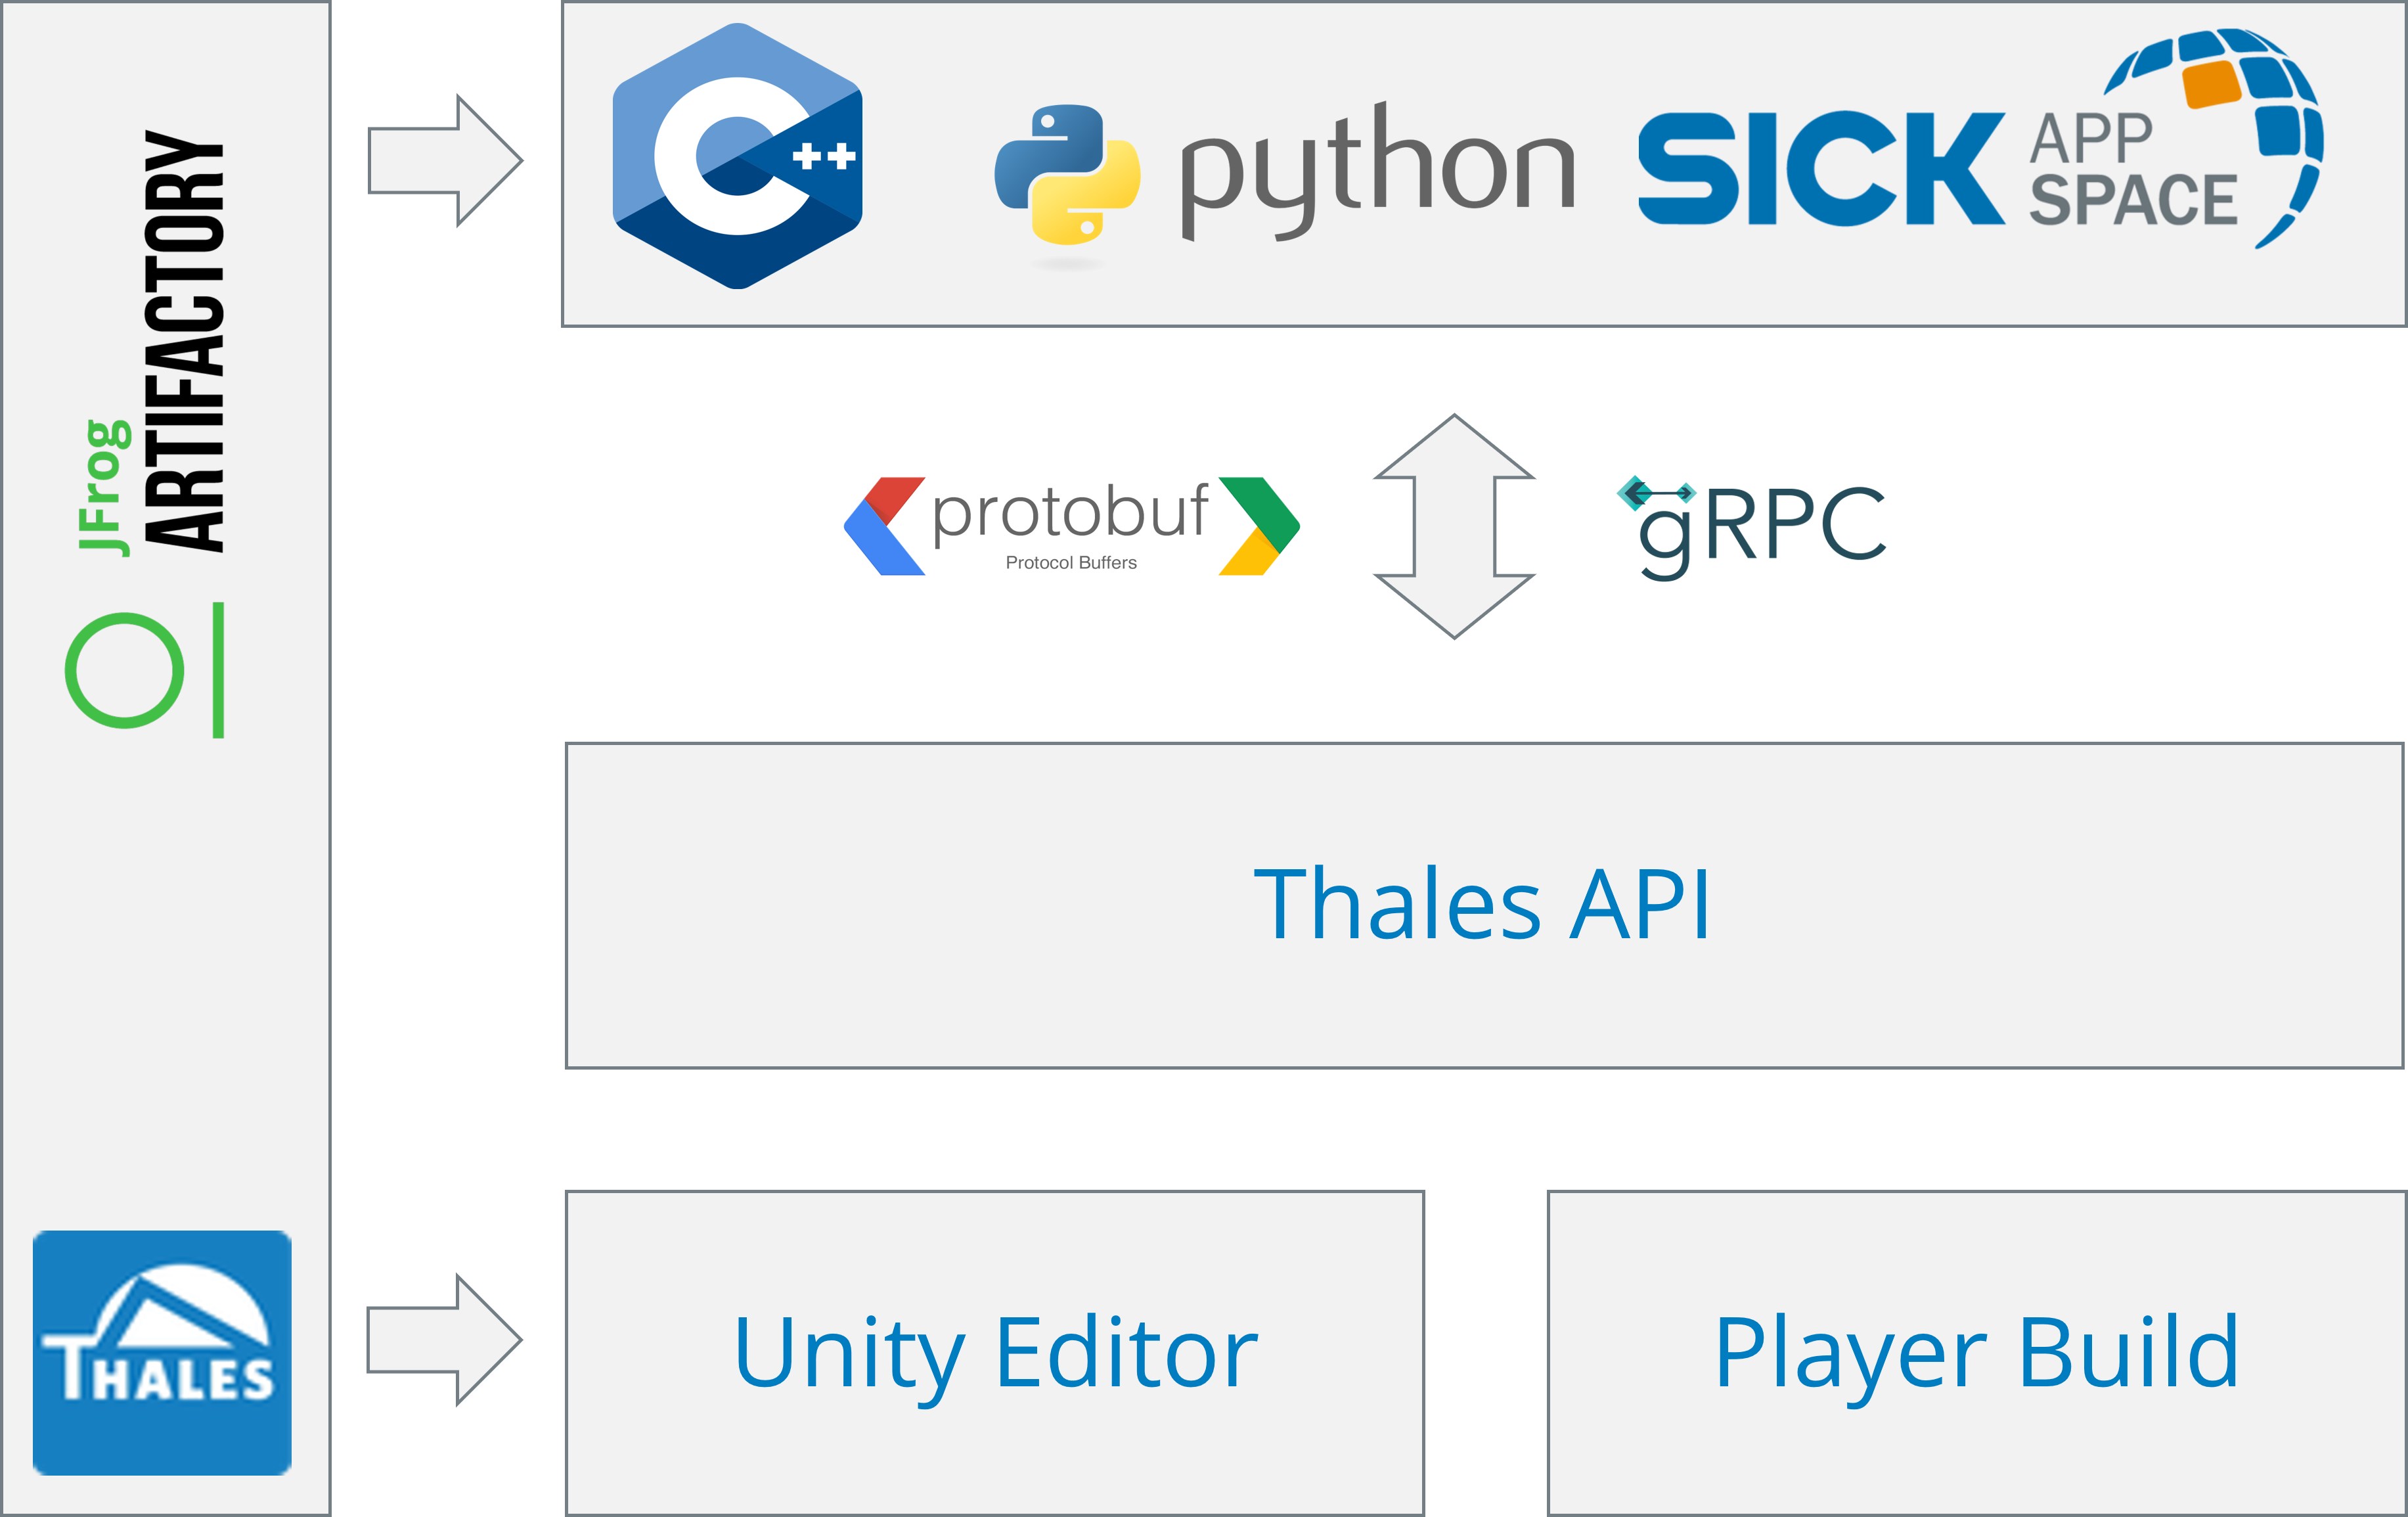
\includegraphics[width=(\textwidth/2)]{images/Thales_Framework.png}
    \caption{Thales Framework}
    \label{fig:Thales-Framework}
\end{figure}


\section{Senoren in der VirtuellenUmgebung}
%Wie funktionieren die Sensoren in Unity?
Im Thales-Paket sind vordefinierte LIDAR-Scanner als Fertigteile enthalten, die mühelos in der entsprechenden Szene instanziiert werden können. Alternativ besteht die Möglichkeit, einen generischen LIDAR-Scanner zu erstellen und entsprechend zu konfigurieren, indem die Systemdiagrammkomponente direkt genutzt wird. Die Nutzung von vorgefertigten Elementen, wie in der Sektion "Spezifische LIDAR-Prefabs" dargestellt, bietet eine zügige und unkomplizierte Möglichkeit, die Arbeit mit virtuellen LIDAR-Sensoren aufzunehmen. Dies erweist sich insbesondere dann als hilfreich, wenn der gewünschte Sensor bereits in Thales verfügbar ist. Falls die Absicht besteht, LIDAR-Scanner zu verwenden, die nicht im bereitgestellten Paket enthalten sind, oder wenn generell LIDAR-Geräte in einem frühen Entwicklungsstadium erforscht werden sollen, bietet es sich an, die generische LIDAR-Scanner-Komponente zu nutzen. Für Fälle, in denen eine raffiniertere Sensormodellierung angestrebt wird, besteht sogar die Möglichkeit, eine individuelle Systemdiagrammkomponente zu erstellen. Referenzimplementierungen hierzu sind in den Systemgraph-Komponenten innerhalb von Thales verfügbar.\\

\begin{figure}[htp]
    \centering
    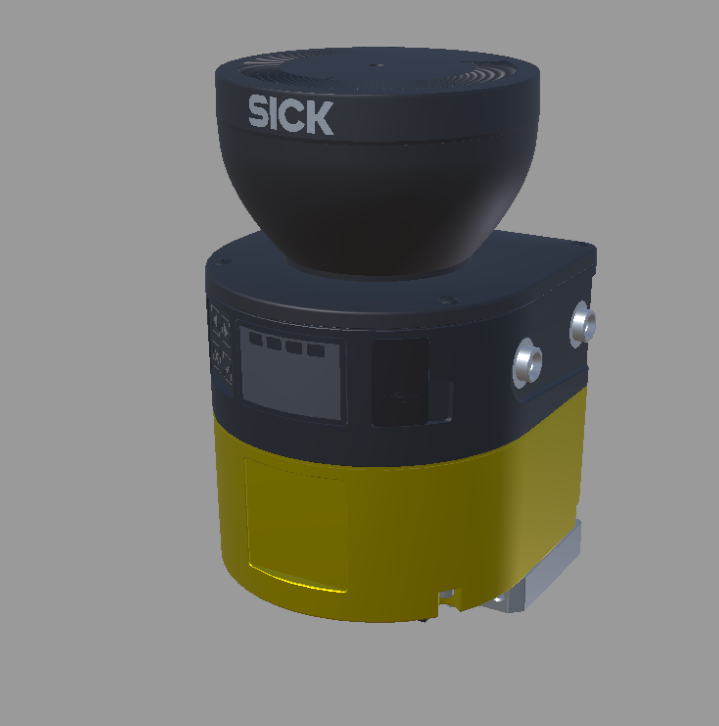
\includegraphics[width=(\textwidth/3)]{images/ModelMircoScan.PNG}
    \caption{MicroScan3}
    \label{fig:MicroScan3}
\end{figure}

\subsubsection*{Rasterisierung basierende LIDAR-Scanner}



Diese Implementierung nutzt Rasterisierungs-Shader als Backend-Technologie und erfordert keine RTX-Hardware. Obwohl es in gewisser Hinsicht seine Grenzen hat, ist es oft eine vernünftige Wahl, insbesondere wenn Sie keine hohe Simulationsgenauigkeit benötigen.\\

\begin{figure}[htp]
    \centering
    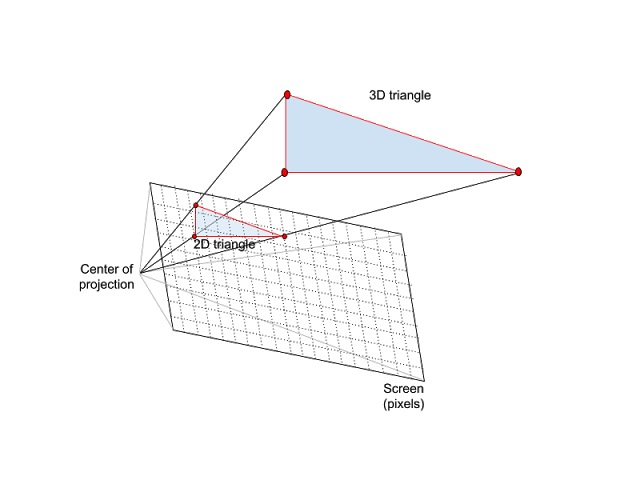
\includegraphics[width=(\textwidth/2)]{images/projection_3d_to_screen.png}
    \caption{Rasterisierung}
    \label{fig:Rasterisierung}
\end{figure}


Bei der Rasterisierung werden die Objekte auf dem Bildschirm aus einem Netz virtueller Dreiecke oder Polygone erstellt, die 3D-Modelle von Objekten bilden. In diesem virtuellen Netz überschneiden sich die Ecken jedes Dreiecks - die so genannten Scheitelpunkte - mit den Scheitelpunkten anderer Dreiecke unterschiedlicher Größe und Form. Jedem Scheitelpunkt ist eine Vielzahl von Informationen zugeordnet, darunter seine Position im Raum sowie Informationen über Farbe, Textur und seine "Normale", mit der die Ausrichtung der Oberfläche eines Objekts bestimmt wird.\\
%https://de.wikipedia.org/wiki/Rasterung#:~:text=In%20der%202D%2DComputergrafik%20bezeichnet,einer%20Vektor%2D%20in%20eine%20Rastergrafik. Teile davon kopieren wenn noch Zeit ist
%Wie funktioniert die Raterisierung in diesem Kontext?
%Die Kamera nimmt ein Bild auf und skalliert es runter auf bis aus den Vector grafiken nur noch Pixel zusehen sind. Mit dem Abstand der Pixel kann die Distanz bestimmt werden. so habe ich das verstanden

\begin{figure}[htp]
    \centering
    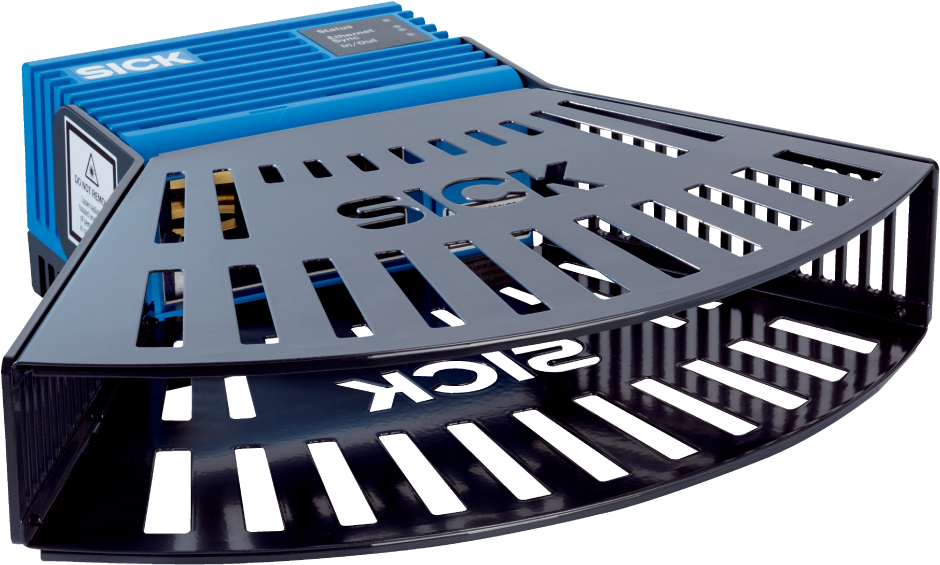
\includegraphics[width=(\textwidth/3)]{images/LMS4000.png}
    \caption{LMS4000}
    \label{fig:LMS4000}
\end{figure}
\subsubsection*{RTX basierende LIDAR-Scanner}
Das RTX-basierte Lidar-Scanner-Modell nutzt Echtzeit-Raytracing und erfordert daher eine Grafikkarte, die RTX unterstützt. Diese Implementierung kann erhalten werden, indem das GenericLidarScannerRTX-Systemdiagramm auswählt wird.\\





%Wie funkt RTX raytracing?
%Es basiert auf raytracing so wie in der realen welt fällt licht auf das object und dann in auf den Sensor so kann der Abstand durch time of light bestimmt werden.

%\chapter{Konzept}
\section{Erstellung der Sensoern in der Virtuellen Umgebung}
\section{AGVs in der Virtuellen Umgebung}
\chapter{Implementierung}
\section{Implementierung der Schnittstelle}
\section{AGVs in der virtuellen Umgebung}
\chapter{Ergebnis}
%Präsentiere deine Forschungsergebnisse in klar strukturierter Form. Verwende Tabellen, Grafiken oder Diagramme, um deine Ergebnisse zu veranschaulichen. Interpretiere die Ergebnisse und beantworte deine Forschungsfragen.

\section{Diskussion}
%Interpretiere deine Ergebnisse im Kontext des theoretischen Hintergrunds. Diskutiere, wie deine Ergebnisse zu den bestehenden Erkenntnissen passen oder davon abweichen. Zeige auf, welche Implikationen deine Arbeit hat und welche offenen Fragen bleiben.
%\section{Notizen}
\subsection{Aufgaben}
Die Aufgabe ist es sich in Unity ein zuarbeiten. Dort eine Scenerie aufzubauen und die Daten die die vier Sensoren liefern mit den Bewegungs vektoren übertragen.
Die übertragung soll über einen gRPC Client und einen gRPC Server laufen. Dannach sollen mit den erzeugten Daten das Feld des DSM Host in Unity angezeigt werden(Best Case für Demo gedacht).
\begin{itemize}
    \item Zeitplan
    \item Riskomanagment
    \item 
\end{itemize}
\subsection{Zeitplan}

\begin{itemize}
    \item 13. Juli - 21. Juli = 7 Tage
    \item 4. September - 30. September = 20 Tage
    \item 27 Arbeitstage a 7 Stunden gleich 189 Stunden
\end{itemize}



% Please add the following required packages to your document preamble:
% \usepackage[table,xcdraw]{xcolor}
% If you use beamer only pass "xcolor=table" option, i.e. \documentclass[xcolor=table]{beamer}

\begin{landscape}
    
\begin{tabularx}{21cm}{|l|l|l|X|X|X|X|X|X|X|X|X|X|X|X|}
    \hline
    \textbf{Aufgabe}                       & \textbf{Anfang} & \textbf{Ende} & \textbf{28}            & \textbf{29}            & \textbf{30}            & \textbf{31}            & \textbf{32}            & \textbf{33}            & \textbf{34}            & \textbf{35}            & \textbf{36}            & \textbf{37}            & \textbf{38}            & \textbf{39}            \\ \hline
    Planung+ Aufgabe Prio 1                & 12.07           & 14.07         & \cellcolor[HTML]{34CDF9} &                          &                          &                          &                          &                          &                          &                          &                          &                          &                          &                          \\ \hline
    Aufgabe Prio 2                         & 17.07           & 21.07         &                          & \cellcolor[HTML]{34CDF9} &                          &                          &                          &                          &                          &                          &                          &                          &                          &                          \\ \hline
    Abwesenheit                            & 24.07           & 01.09         &                          &                          & \cellcolor[HTML]{C0C0C0} & \cellcolor[HTML]{C0C0C0} & \cellcolor[HTML]{C0C0C0} & \cellcolor[HTML]{C0C0C0} & \cellcolor[HTML]{C0C0C0} & \cellcolor[HTML]{C0C0C0} &                          &                          &                          &                          \\ \hline
    Aufgabe Prio 2                         & 04.09           & 08.09         &                          &                          &                          &                          &                          &                          &                          &                          & \cellcolor[HTML]{34CDF9} &                          &                          &                          \\ \hline
    Aufgabe Prio 3                         & 11.09           & 15.09         &                          &                          &                          &                          &                          &                          &                          &                          &                          & \cellcolor[HTML]{34CDF9} &                          &                          \\ \hline
    Aufgabe Prio 4+Doku                    & 18.09           & 29.09         &                          &                          &                          &                          &                          &                          &                          &                          &                          & \cellcolor[HTML]{68CBD0} & \cellcolor[HTML]{68CBD0} & \cellcolor[HTML]{68CBD0} \\ \hline
    Praxisbericht + Kollogium Vorbereitung & 18.09           & 22.09         &                          &                          &                          &                          &                          &                          &                          &                          &                          &                          & \cellcolor[HTML]{34FF34} &                          \\ \hline
    Kollogium                              & 25.09           & 29.09         &                          &                          &                          &                          &                          &                          &                          &                          &                          &                          &                          & \cellcolor[HTML]{FE0000} \\ \hline
\end{tabularx}
\end{landscape}
   

\subsection{Notizen 03.07}
Unity zum laufen bekommen auf dem anderen PC.


\subsection{Themenbesprechung Protokoll}
Welche Scenarian sind reelevant?
Vergleich zwischen Unity und Ross
Zeitplan erstellen
Aufgabenpakte erstellen
Riskomodelle
Riskoeinschätzung
Was kann schief gehen?
EIn kapitel Riskomanament
Ein kapitel Zeitplan Arbietspakete
Problemstellung verstehen
Schutzfelder nicht
ein zwei Wochen Arbeitspakete
Wochen Meeting
Jira nach Zeitplan füllen
Zeit ein planen zum Bericht schreiben jeden Tag eine Stunde 


Prios der arbeit
Prio 1 Senordaten über gRPC übertragen
Prio 2 Wenderadius und Geschwindigkeit übertragen mit der Thales (Einauto selbst Desginen)
es gibt mehrer auto: gabelstapler, Panzerrolle, normale Auto
Prio 3 Polghonzug erhalten und in Unity darstellen
Prio 4 NotSignal erhalten und das AGV anhalten 
Prio 5 Beispiel Scene zu Sever Client wo die Daten von einem Sensor übertragen werden. Dann auch noch die Parameter von einem Template GameObject übertragen wird.


\subsection{12.07}
Plan für heute dem AGV Geschwindigkeit geben. Und weiter geben. Das Problem die AGV/Service wird nicht erkannt. Obwohl der SplineWalker mit dem dem Agv Service Script verbunden ist. Die 

\subsection{13.07}
\begin{itemize}
\item Projekt Einsicht in VS Studio
\item Martin schreiben wegen dem AGV übertragung
\item Fragen formulieren zur Thales Schnittstelle
\item 
\end{itemize}

Fragen zur Thales Schnittstelle
\begin{itemize}
\item Jan hat eine Agvservice script erstellt welches IAgv verwendet aber es wird nicht bei den Avalibele Services angezeigt
\item Hallo Martin wir haben noch ein paar Fragen zur Thales Api. Hast du heute Nachmittag Zeit für ein Meeting mit Artem und mir?
\end{itemize}

\subsection{14.07}
\begin{itemize}
\item Sprint Meeting vorbereiten
\item die vier Scanner abfragen und übertragen. Wie funktioiert das mit dem Stepper?
\item Welche Scanner sollen übertragen werden?
\item Wie werden AGVs in Unity umgesetzt?
\item Aufgaben in Jira 
\end{itemize}

\subsection{17.07}
\begin{itemize}
\item Doku erledigt
\item Nächste Aufgabe erstellen es AGV
\end{itemize}

Nächste Aufgabe erstellen es AGV
\begin{itemize}
\item Scene aufbauen
\item Object für des AGV erstellen 
\end{itemize}

\subsection{18.07}
Aufgaben für heute 
\begin{itemize}
\item Inhaltsverzeichnis für Bericht erstellen
\item Git zum laufen bringen 
\item Arbeitsparkte für AGVs erstellen
\end{itemize}

%\include{input/kapitel1}
%\include{input/kapitel2}

% Ab hier beginnt der Anhang

\pagenumbering{Roman}
\setcounter{page}{\value{savepage}}

\addcontentsline{toc}{chapter}{Anhang}

\addcontentsline{toc}{chapter}{Index}
\printindex

\addcontentsline{toc}{chapter}{Literaturverzeichnis}

% Haben Sie das "biblatex"-Paket nicht installiert, benutzen Sie folgendes:
% Ohne das "biblatex"-Paket (s. bericht.sty) produziert folgendes
% "deutsche" Zitate in Literaturverzeichnissen gemaß der Norm DIN 1505,
% Teil 2 vom Jan. 1984.
% Die Zitatmarken werden alphabetisch nach Verfassern
% sortiert und sind durch abgekürzte Verfasserbuchstaben plus
% Erscheinungsjahr in eckigen Klammern gekennzeichnet.

% \bibliographystyle{alphadin}
% \bibliography{bericht}

%%%%%%%%%%%%%%%%%%%%%%%%%%%%%%%%%%%%%%%5
% BIBLATEX
% Benutzt man das "biblatex"-Paket, muß man folgendes schreiben:
\def\refname{Literaturverzeichnis}
\printbibliography
%%%%%%%%%%%%%%%%%%%%%%%%%%%%%%%%%%%%%%%5


%%%%%%%%%%%%%%%%%%%%%%%%%%%%%%%%%%%%%%%%%%%%%%%%%%%%%%%%%%%%%%%%%%%%%%%%%%%%%%%
%% Descr:       Vorlage für Berichte der DHBW-Karlsruhe, Änderungshistorie
%% Author:      Prof. Dr. Jürgen Vollmer, vollmer@dhbw-karlsruhe.de
%% $Id: changelog.tex,v 1.16 2020/03/13 15:12:39 vollmer Exp $
%% -*- coding: utf-8 -*-
%%%%%%%%%%%%%%%%%%%%%%%%%%%%%%%%%%%%%%%%%%%%%%%%%%%%%%%%%%%%%%%%%%%%%%%%%%%%%%%

\chapter*{Änderungen}

\begin{description}
\item[2020/03/13] Tippfehler korrigiert\\
                  aktuelle Formulierungen aus der Prüfungsordnung Technik übernommen\\
                  Formatdatei erklärt
\item[2017/10/06] Anpassung an neuer Versionen diverse Pakete.
\item[2016/03/16] Auf UTF-8 umgestellt, Indices.
\item[2010/04/12] ToDo-Markierungen mit dem \verb+\todo+-Kommando.
\item[2010/01/27] Anhang (\texttt{appendix}), Selbständigkeits-Erklärung, \texttt{framed}-Paket.
\item[2010/01/21] Abkürzungen (\texttt{acronym}), \texttt{table} und \texttt{tabular} benutzt,
     unübliche Pakete beigelegt.
\item[2010/01/18] Code-Listings (\texttt{listings}), Literaturreferenzen \texttt{biblatex})
\item[2010/01/11] Initiale Version.
\end{description}


\newpage
\addcontentsline{toc}{chapter}{Liste der ToDo's}
\listoftodos[Liste der ToDo's]


\end{document}
